% \subsection{EMBERS Introduction}
\begin{frame}{Studying Model-drift in Anticipatory Intelligence Systems}
\begin{itemize}
    \item EMBERS Introduction
    \item EMBERS Performance
    \item Ablation Testing
    \item EMBERS Successes and Misses
    \item Uncertainty in forecasting
    \item Model Drift
\end{itemize}
    
\end{frame}
\begin{frame}{EMBERS Introduction}
EMBERS - Early Model Based Event Recognition using Surrogates
    \begin{itemize}
        \item 24x7 continuous forecasting system
        \item Deployed - Nov 2012 
        \item Aims to develop methods for continuous, automated analysis of publicly available data in order to anticipate and/or detect population-level events
        \item Event classes 
            \begin{itemize}
                \item Civil Unrest, Rare Diseases, Influenza Like Illness, Elections, Domestic Political Crises
            \end{itemize}
        \item ~\cite{kdd:beating-the-news, doyle2014forecasting, zhao2014unsupervised} ...
    \end{itemize}
\end{frame}

% \subsection{EMBERS Performance}
\begin{frame}{EMBERS Performance}
\begin{figure}
    \centering
    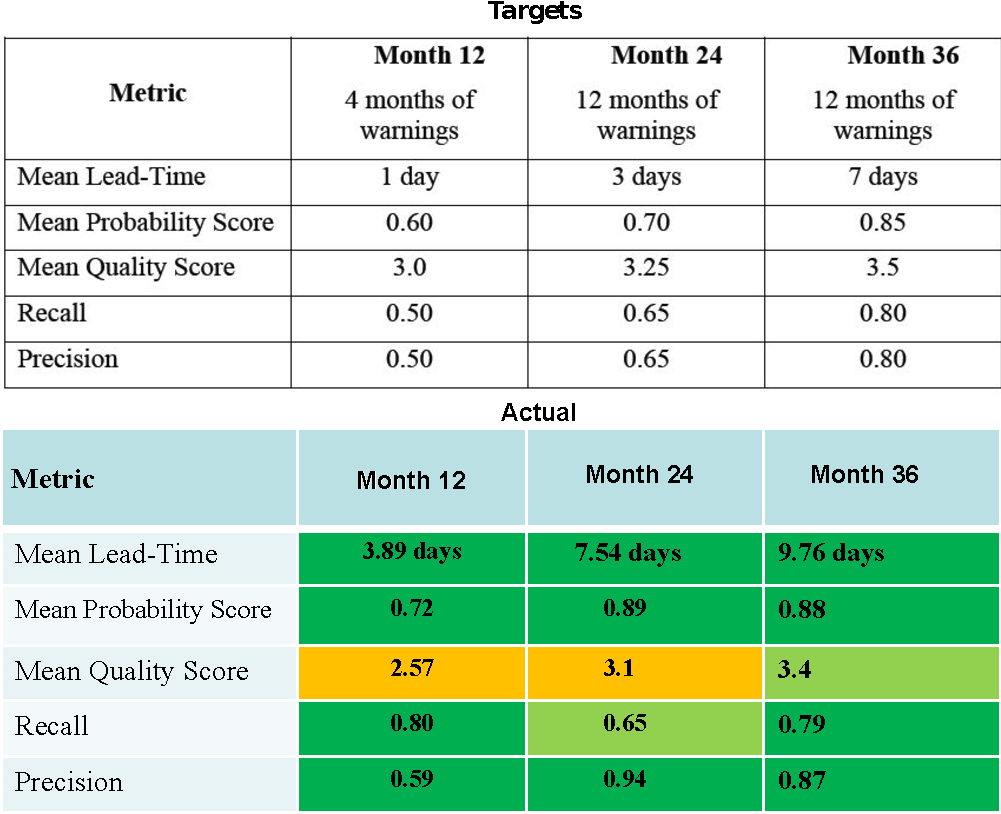
\includegraphics[width=0.7\textwidth]{Problem1/figures/performance_tb1.pdf}
    \label{fig:my_label}
\end{figure}
\end{frame}

\begin{frame}{EMBERS Introduction (Contd.)}
    Data Sources
    \begin{itemize}
        \item Social Media sources: Twitter, Facebook events
        \item Traditional Media: News, Blogs
        \item Historical events: ICEWS~\cite{boschee2015icews}, GDELT~\cite{leetaru2013gdelt}
        \item Numerical - Tor, stock/currency exchange values
    \end{itemize}
    
    % Models
    % \begin{itemize}
    %     \item Dynamic Query Expansion, Planned Protest, Volume based model, MLE, BaseRate etc
    % \end{itemize}
\end{frame}

% \subsection{Ablation Testing}
\begin{frame}{Ablation Testing}

\begin{table}
\resizebox{\columnwidth}{!}{
\begin{tabular}{l|cccc}
\toprule
Data Source          & Quality-Score & Lead-time & Precision & Recall \\
\midrule
Removing news and blogs & -16.48\% &-55\% &+35\% &-14\% \\

Removing social media & +8.42\% & +30\%  &+79\% &-33\% \\
\bottomrule
\end{tabular}
}
\end{table}

\pause
\begin{itemize}
    \item Social media sources provide high recall \pause
        \begin{itemize} 
            \item Daily chatter/discussion 
        \end{itemize}
    \item High lead-time from traditional sources \pause
        \begin{itemize}
            \item Planned Protests are generally reported in traditional media
        \end{itemize}
\end{itemize}
\end{frame}


% \subsection{EMBERS Successful forecasts}
\begin{frame}{Successful Forecasts}
\begin{center}
\small
    Paraguay Protests Feb. 2015
\end{center}
\vspace{-1em}

\begin{tikzpicture}
\begin{scope}[xshift=6cm]
    \node[anchor=south west,inner sep=0] (image) at (0,0) {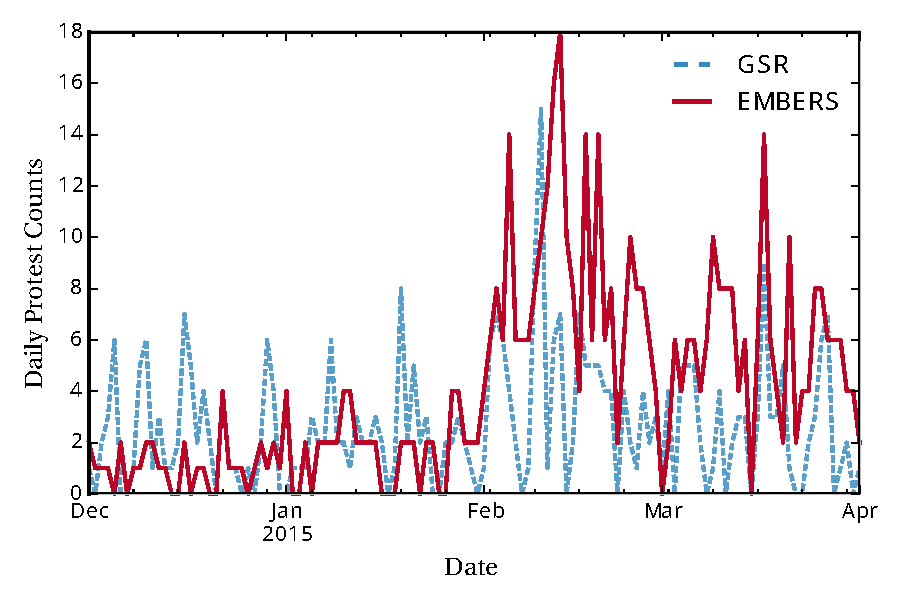
\includegraphics[width=0.5\textwidth]{Problem1/figures/paraguayFeb15.pdf}};
    \begin{scope}[x={(image.south east)},y={(image.north west)}]
        % \draw[red,ultra thick] (0.48,0.80) ellipse (0.55,0.95);
        \draw[green,ultra thick] (0.6,0.50) ellipse (1cm and 2cm) node(peak){};
    \end{scope}
\end{scope}
\node [anchor=west] (note) at (1,3) {{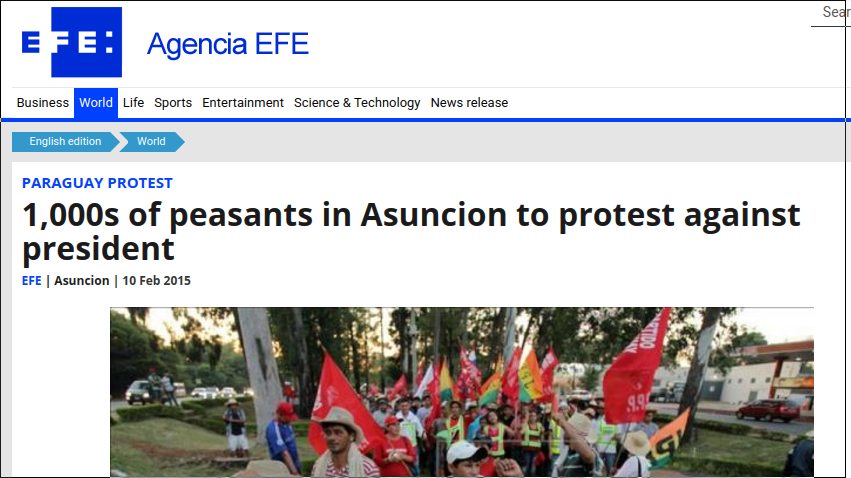
\includegraphics[width=0.3\textwidth]{Problem1/figures/peasants.png}};};

\path[->,green,thick] (note) edge [bend right] (peak);
\end{tikzpicture}%
\vspace{-1em}
\pause

Some more examples:
\begin{itemize}
\small
    \item Brazilian Spring (June 2013)
    \item Venezuelan Protests (Feb-March 2014)
    \item Mexico (Oct 2014)
    \item Colombia (Dec'14-March 2015)
\end{itemize}
\end{frame}


% \begin{frame}{Frame Title}
    
% % \begin{figure}[h!t]

% % \begin{annotatedFigure}
% % 	{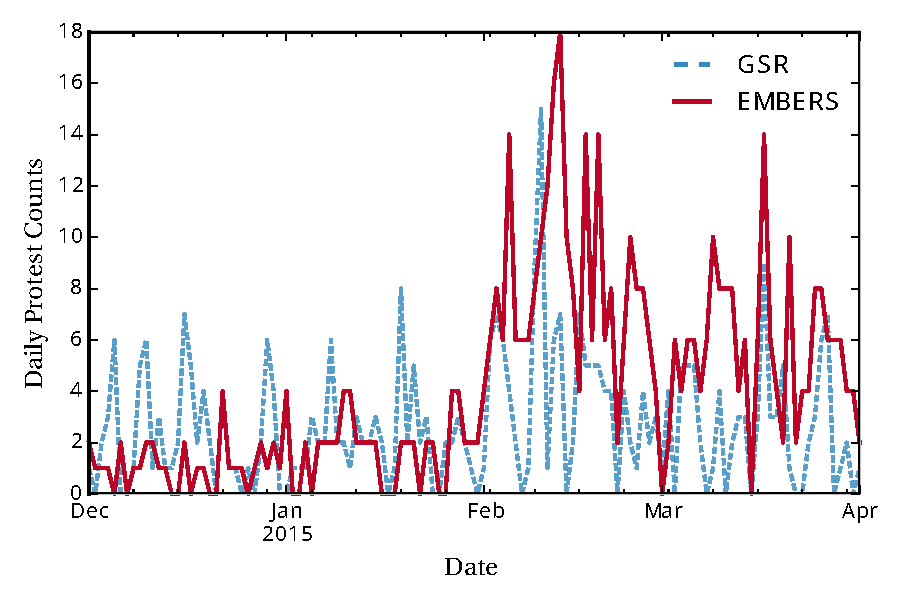
\includegraphics[width=0.8\linewidth]{Problem1/figures/paraguayFeb15.pdf}}\pause
% % 	\annotatedFigureBox{0.4995,0.2514}{0.731,0.9505}{A}{0.4995,0.2514}%bl
% % \end{annotatedFigure}

% % \end{figure}

% \begin{tikzpicture}
% \begin{scope}[xshift=1.5cm]
%     \node[anchor=south west,inner sep=0] (image) at (0,0) {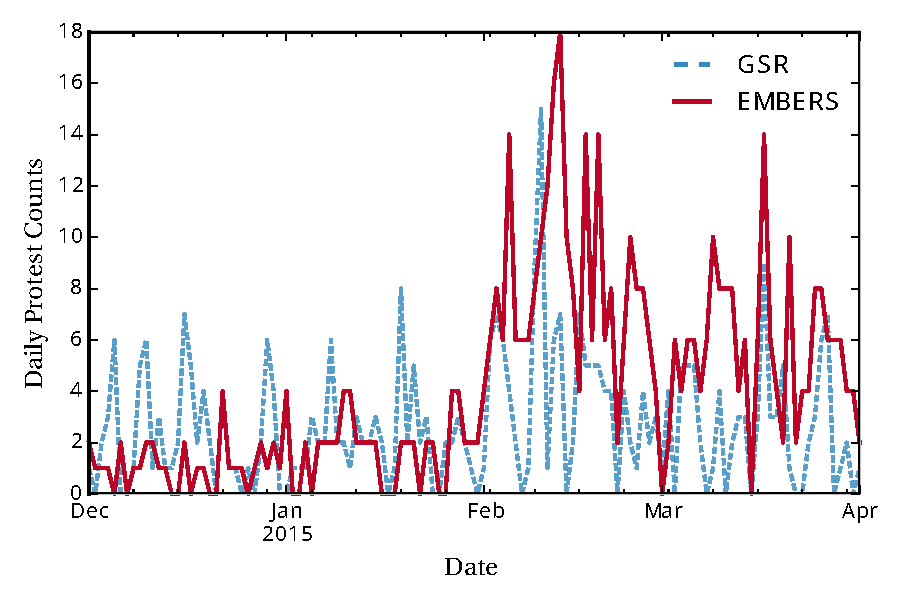
\includegraphics[width=0.5\textwidth]{Problem1/figures/paraguayFeb15.pdf}};
%     \begin{scope}[x={(image.south east)},y={(image.north west)}]
%         % \draw[red,ultra thick] (0.48,0.80) ellipse (0.55,0.95);
%         \draw[green,ultra thick] (0.6,0.50) ellipse (1cm and 4cm) node(peak){};
%     \end{scope}
% \end{scope}
% \node [anchor=west] (note) at (1,5) {{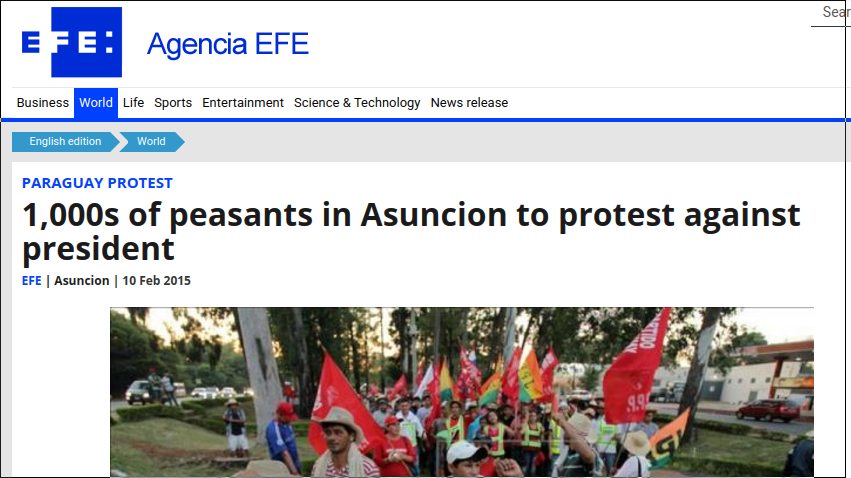
\includegraphics[width=0.3\textwidth]{Problem1/figures/peasants.png}};};

% \path[->,green,thick] (note) edge [bend right] (peak);
% \end{tikzpicture}%


% \end{frame}



% \subsection{EMBERS Misses}
\begin{frame}{EMBERS Misses}
\begin{center}
    Mexico 2014
\end{center}
    \begin{figure}
        \centering
        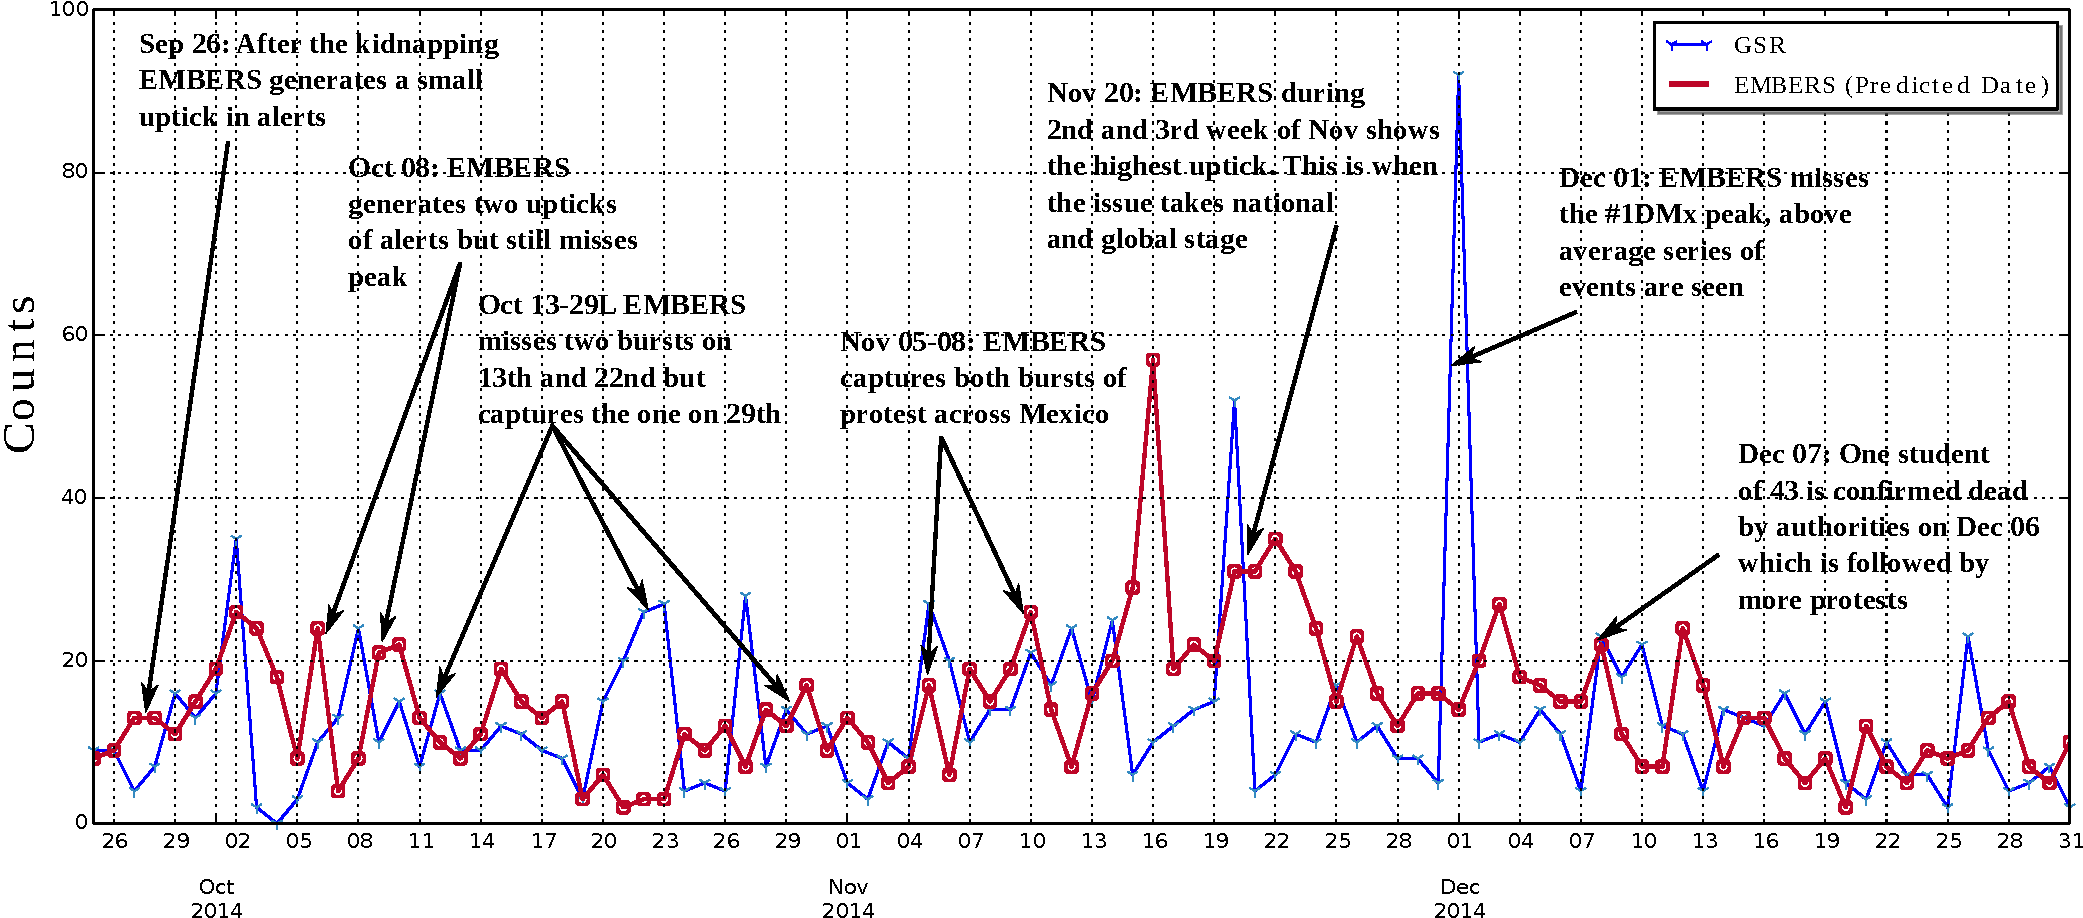
\includegraphics[width=\textwidth]{Problem1/figures/mx_timeline.pdf}
    \end{figure}
\end{frame}

% \subsection{Uncertainty in Forecasts}
   \begin{frame}{Uncertainty in Forecasting}
       
    \begin{figure}
        \centering
        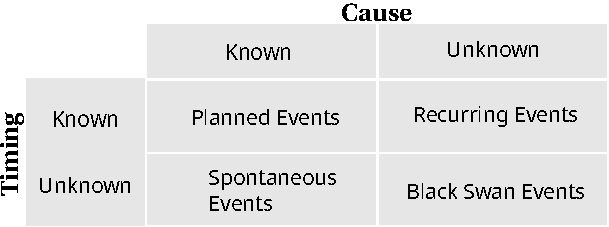
\includegraphics[width=\textwidth]{Problem1/figures/event_confusionMatrix.pdf}
    \end{figure}
    \end{frame}

% \subsection{Model Drift}
\begin{frame}{Model Drift}
\begin{figure}
    \centering
    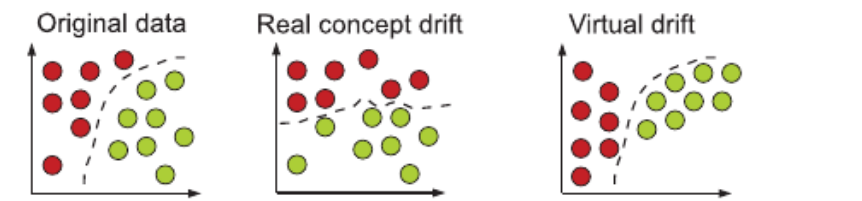
\includegraphics[width=0.9\textwidth]{Problem1/figures/modelDrift.png}
    \caption{Gama et al.,~\cite{gama2014survey}}
\end{figure}
\vspace{-1em}
Broadly defined as change in data-target relationship over time \\
Kinds of drift
\begin{itemize}
    \item \textit{Input(or Target) data drift}: only $P(x)$ changes not $P(y|x)$. Example-Change in twitter volume over time
    \item \textit{Input-Target Drift}: Relationship between input and target changes over time
\end{itemize}
\end{frame}


\begin{frame}{Model Drift in EMBERS}
Possible reasons
\begin{itemize}
    \item<1->Significant change in event landscape
    \begin{itemize}
        \item<2-> Change in rate of events 
        \only<2->{
                 \begin{figure}
                    \centering
                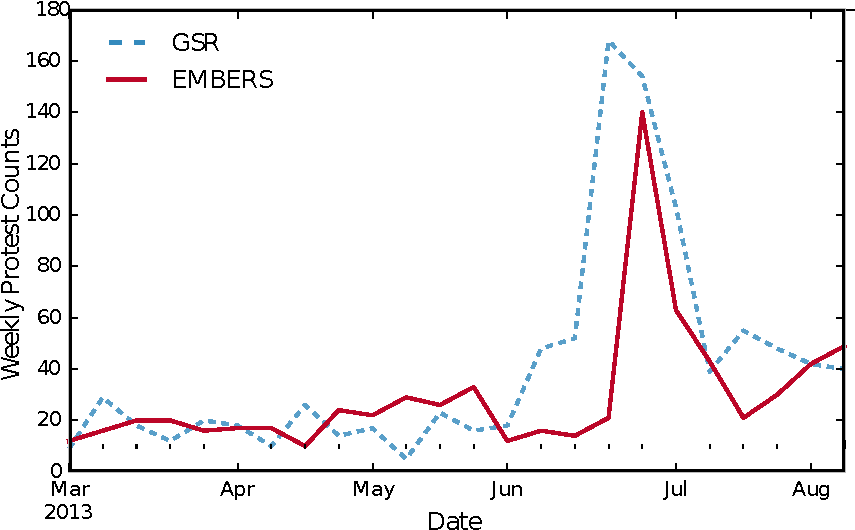
\includegraphics[width=0.5\textwidth]{Problem1/figures/brazilJune13.pdf}
                \end{figure}
                }
        % \item Example: Government instability can cause lead to increase in number of protests
    \end{itemize}
    \item<3-> Data sources becoming obsolete (or arrival of New data sources)
        \begin{itemize}
            \item Black swan events (unknown-unknowns)
        \end{itemize}
\end{itemize}
\end{frame}


\begin{frame}{Model drift Adaptation - Steps involved}
Three main steps:
\begin{itemize}
    \item Concept Drift Detector
    \begin{itemize}
        \item Near real-time source of GSR needed
            \begin{itemize}
                \item EMBERS AutoGSR~\cite{saraf2016embers}
            \end{itemize}
        \item HQCD~\cite{chakraborty2016hierarchical}, BOCPD~\cite{adams2007bayesian} etc
    \end{itemize} \pause
    \item Real-time Parameter tuning based on updated estimate of expected rate of events for time $t+1$
    \begin{itemize}
        \item Quality score threshold in EMBERS suppressor
            \begin{itemize}
                \item update threshold based on (1) estimated rate of events, (2) expected number of alerts and (3) suppressor quality score density distribution
            \end{itemize}\pause
        \item Rate-Adapted BaseRate
        \begin{itemize}
            \item Sample events at random from past month to account for difference in rate
        \end{itemize}
    \end{itemize}\pause
    \item Model re-training after enough data is accumulated from post-change distribution
\end{itemize}
    
\end{frame}

\subsection{Model drift Adaptation Framework}
\begin{frame}{Model drift Adaptation Framework}
    \begin{figure}
        \centering
        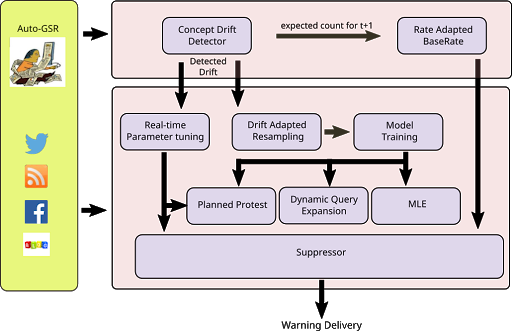
\includegraphics[width=0.8\textwidth]{Problem1/figures/driftAdaptationFramework.png}
    \end{figure}
\end{frame}

% \subsection{Model Drift Experiment settings}
\begin{frame}{Model drift Experiments}
\begin{itemize}
    \item \textbf{\textit{Monthly trained}}: All models for month `$n$' are trained with data upto `$n-1$'
    \item \textbf{\textit{6 months old}}: Models trained using data upto `$n-6$' data and no drift correction done
    \item \textit{\textbf{EMBERS delivered}}: Set of delivered EMBERS alerts
    \item \textit{\textbf{Drift Corrected}}: Models are adapted if and only if a drift is detected
\end{itemize}
\end{frame}




% \subsection{Model Drift Results}
\begin{frame}{Model Drift Results}
\vspace{-1em}
\begin{table}
\scriptsize
\begin{tabular}{p{1.5 cm}p{2cm}rrrrrrrrrrr}
\toprule
& & LS &  DS &  ES &  PS &  QS &  Prob-M &  LT &  Prec. &  Recall \\
\midrule
\textbf{Venezuela} &   Monthly Trained  & \textbf{0.90} &    0.94 &    0.58 &    \textbf{0.39} &   \textbf{ 3.69} &        \textbf{0.89} &    \textbf{5.01} &       \textbf{0.93} &    0.60 \\
         &      6 months old   & 0.88 &    0.94 &    \textbf{0.60} &    \textbf{0.39} &    3.64 &        0.88 &    2.93 &       0.92 &    0.49 \\
         &  EMBERS-delivered   & 0.88 &    \textbf{0.95} &    0.58 &    0.38 &    3.64 &        0.87 &    4.53 &       0.91 &    0.50 \\
         &   Drift Corrected   & 0.84 &    0.90 &    0.59 &    0.34 &    3.48 &        0.86 &    3.99 &       0.88 &    \textbf{0.75} \\
\midrule
\textbf{Brazil}   &   Monthly Trained   & 0.88 &    0.89 &    \textbf{0.48} &    0.42 &    3.54 &        0.73 &    \textbf{6.98} &       0.60 &    0.51 \\
         &      6 months old   & 0.86 &    0.87 &    0.46 &    0.49 &    3.46 &        \textbf{0.77} &    3.46 &       \textbf{0.75} &    0.37 \\
         &  EMBERS-delivered   & 0.87 &    0.88 &    0.47 &    \textbf{0.52} &    3.49 &        \textbf{0.77} &    5.89 &       0.73 &    0.51 \\
         &   Drift Corrected   &\textbf{0.89} &    \textbf{0.89} &    0.47 &    0.42 &    \textbf{3.55} &        0.76 &    5.27 &       0.66 &    \textbf{0.60} \\
\bottomrule
\end{tabular}
\end{table}

\begin{itemize}
\small
    \item Regular training shows higher lead-time
    \item Quality does not improve much with regular re-training
    \item Recall improves with regular re-training
    \item Drift correction helps improve recall with minor\\ sacrifice in precision (and QS w.r.t to venezuela)
\end{itemize}
\end{frame}

\begin{frame}{Takeaways}
\begin{itemize}
    \item Ground truth definition/ quality/ granularity(specificity) has big impact on model performance
    \item Single OSI source may be noisy/unreliable
    \item Model-drift is a major issue
        \begin{itemize}
            \item Near-real time source of Ground-Truth necessary for timely change detection
            \item Real-time parameter tuning necessary for updating models
        \end{itemize}
\end{itemize}
    
\end{frame}